\chapter{Learning Algorithms}

Equipped with the theoretical frameworks from the previous chapter, we are now going to look at several algorithms which can be used to construct machines that learn.

We distinguish between two phases in the lifecycle of an AI model:
\begin{itemize}
    \item \emph{Training}: processing the available training data or interacting with the environment until a satisfactory learning performance is reached.
    \item \emph{Inference}: using the trained model to perform predictions on previously unseen data or to interact with the environment in new scenarios.
\end{itemize}
We will judge the algorithms both from the perspective of how many resources and time they require during training, as well as with regards to their efficiency and accuracy during inference.

\section{Linear Regression}

In a data modelling problem, the simplest hypothesis we can use (excluding a constant function) is a \emph{linear function}:
\[
    h(x) = A x + b
\]
    where \(A \in \reals^{1 \times n}\) is a row-matrix of coefficients and \(b\) is a free coefficient, usually called \emph{bias}.

\subsection{Least Squares Regression}

One of the oldest methods for performing linear regression is the \emph{method of least squares}. This has been known for over 300 years, since the times of Legendre and Gauss, who used it to analyse the orbit of celestial objects. The formulation described below is inspired by the one in \cite{Mohri2018}.

Let \(X\) be the input space and suppose that we have a function \(\varphi \colon X \to \reals^d\), called the \emph{feature map}, which provides an embedding of our data into Euclidean space. As mentioned above, we will work with the following hypothesis set:
\[
    H = \Set{ h \colon \reals^d \to \reals | h(x) = a x + b, a \in \reals^d, b \in \reals }  
\]

Given a sample of training data \(\left(x_1, y_1\right), \dots, \left(x_n, y_n\right)\), the empirical risk using the \emph{mean squared error} loss function is:
\begin{align*}
    \widehat{R} (h) &= \frac{1}{n} \sum_{i = 1}^{n} \left(h(\varphi\left(x_i\right)) - y_i \right)^2 \\
    &= \frac{1}{n} \sum_{i = 1}^{n} \left(a \cdot \varphi\left(x_i\right) + b - y_i \right)^2
\end{align*}

We want to find the linear model which minimizes the empirical risk:
\[
    \widehat{h} = \argmin_{h \in H} \widehat{R} (h)
\]

To simplify the problem, let us introduce a few bits of notation. Define the \emph{weight vector} \(W\), the \emph{input matrix} \(X\) and the \emph{targets vector} as
\[
    W = \begin{pmatrix}
        a_1 \\
        \vdots \\
        a_d \\
        b
    \end{pmatrix} \in \reals^{d + 1}
    \quad
    X = \begin{pmatrix}
        \varphi\left(x_1\right) & \cdots & \varphi\left(x_n\right) \\
        1 & \cdots & 1
    \end{pmatrix} \in \reals^{(d + 1) \times n}
    \quad
    Y = \begin{pmatrix}
        y_1 \\
        \vdots \\
        y_n
    \end{pmatrix} \in \reals^{n}
\]
The empirical risk functional becomes
\[
    \widehat{R}'(W) = \frac{1}{n} \norm{X^T W - Y}^2
\]
We remark that the function \(W \mapsto X^T W - Y\) is affine and smooth, while the squared norm function \(\norm{\cdot}^2\) is smooth and convex. Hence, by Fermat's theorem, the global minimum is attained for
\[
    \nabla_{W} \widehat{R}'(W) = 0
\]
which is the solution of
\[
    \frac{1}{n} \cdot 2 X \left(X^T W - Y\right) = 0 \iff X X^T W = X Y
\]
If the matrix \(X X^T\) is invertible, the unique solution is given by
\[
    W = \left(X X^T\right)^{-1} X Y = \left(X^T\right)^{-1} X^{-1} X Y = \left(X^T\right)^{-1} Y
\]
Otherwise, approximative solutions can be obtained by computing a \emph{Moore-Penrose pseudo-inverse} of \(X X^T\).

% \subsection{Logistic Regression}

% Linear regression works well when we want to fit a linear model between several independent variables and the target one. But what if the target variable is not a real number, but rather constrained to be a binary yes/no possibility?

% TODO

% \subsection{Generalized Linear Model}

% It turns out that both linear regression and logistic regression can be integrated in a more general theoretical framework, that of a \emph{generalized linear model}.

% TODO

\section{Kernel Methods}

The term ``kernel'' comes from analysis, where it is used to denote functions which get multiplied with other functions inside an integral in order to map from one function space to another. The general form of an integral transform operator would be
\[
    \left(T \, f\right) (s) = \int_{x_0}^{x_1} \, f(x) \, K(x, s) \diff x
\]
where \(K\) is the \emph{kernel function} associated to this transform.

For example, taking \(K\) to be the function \(e^{-2 \pi i x s}\), we can recover the classical Fourier transform:
\[
    \left(\symcal{F} \, f\right) (s) = \int_{\reals} \, f(x) \, e^{-2 \pi i x s} \diff x
\]

% TODO: find some reference for this integral transform formula, other than Wikipedia: https://en.wikipedia.org/wiki/Integral_transform

% TODO: maybe also give an example with the heat kernel? https://en.wikipedia.org/wiki/Heat_kernel
% Or even the Dirichlet/Fejer kernels? https://en.wikipedia.org/wiki/Dirichlet_kernel

In machine learning, kernels are functions used to replace the usual dot product in the Euclidean space the data lives in. They compute the value of the scalar product between their inputs \emph{as if} they were lifted to some higher-dimensional (possibly even infinite-dimensional) vector space, without actually performing such an embedding. By using them correctly, we are able to transform the initial data such that distinct classes become linearly separable, hence amenable to simple and efficient learning algorithms.

\subsection{Positive-Definite Kernels}

A special class of kernel functions first arose in Hilbert's work on Fredholm integral equations \cite{Hilbert1904_Part1, Hilbert1904_Part2}. Hilbert was interested in finding functions \(\varphi \colon [a, b] \to \reals\) for which
\[
    f(s) = \int_{a}^{b} K(s, t) \varphi(t) \diff t
\]
where \(K\) was called the \emph{kernel} or \emph{nucleus} of the integral equation. More precisely, while analysing \emph{Fredholm equations of the second kind},
\[
    f(s) = \varphi(s) - \lambda \int_{a}^{b} K(s, t) \varphi(t) \diff t
\]
he eventually considered the quantity
\[
    J(\omega) = \int_{a}^{b} \int_{a}^{b} K(x, y) \, \omega(x) \omega(y) \diff x \diff y
\]
defined for any \(\omega \colon [a, b] \to \reals\) satisfying
\[
    \int_{a}^{b} \left(\omega(x)\right)^2 \diff x = 1
\]
(nowadays we would describe such \(\omega\) as having an \(L^2 \left([a, b]\right)\)-norm equal to \(1\)). Hilbert called a kernel \emph{definite} if \(J(\omega)\) is strictly positive, for any continuous real-valued function \(\omega\) (which is not identically zero).

The British mathematician James Mercer built upon Hilbert's work, performing an in-depth analysis of positive-definite kernels and their properties \cite{Mercer1909}.

\begin{definition}
A \emph{positive-definite kernel} on a set \(X\) is a symmetric function \(K \colon X \times X \to \reals\) for which
\[
    \sum_{i = 1}^{n} \sum_{j = 1}^{n} K(x_i, x_j) c_i c_j \geq 0
\]
for any \(n \in \naturals^*\) and any finite sequences \(x_1, \dots, x_n \in X\) and \(c_1, \dots, c_n \in \reals\), with equality iff \(c_1 = c_2 = \dots = c_n = 0\).
\end{definition}

\subsection{Reproducing Kernel Hilbert Spaces}

In the sequel, \(H\) will denote a Hilbert space whose element are \emph{functions} from some fixed set \(X\) to the real numbers \(\reals\).

\begin{definition}
For any point \(x \in X\), the \emph{evaluation functional} \(E_x\) is the map taking an element \(f \in H\) to its value at \(x\), i.e.\
\[
    E_x \left(\, f \right) = f(x)
\]
\end{definition}

\begin{remark*}
Now it should be clear why we choose to work with Hilbert spaces consisting of (genuine) functions. For example, it wouldn't make sense to consider an evaluation functional on \(L^2 (X)\), the space of square-integrable functions on the set \(X\), since its elements are \emph{equivalence classes} of functions, uniquely identified up to sets of null measure. For any \(\widehat{f} \in L^2 (X)\), we can find a representative \(f \in \widehat{f}\) such that \(f(x)\) takes any prescribed value, making \(E_x \left(\, \widehat{f} \right)\) ill-defined.
\end{remark*}

\begin{definition}
The Hilbert space \(H\) is called a \emph{reproducing kernel Hilbert space} if for every \(x \in X\) the evaluation functional \(E_x\) is continuous.
\end{definition}

We will usually abbreviate this term using the initialism ``RKHS''.

Since \(E_x\) is continuous, by the Riesz representation theorem we have that there exists a unique function \(K_x \in H\) such that
\[
    E_x \left(\, f \right) = f(x) = \innerproduct{f}{K_x}
\]
This leads us to the following definition:
\begin{definition}
The \emph{reproducing kernel} of \(H\) is the continuous map
\begin{align*}
    K \colon X \times X &\to \reals \\
    K (x, y) &= \innerproduct{K_x}{K_y}
\end{align*}
\end{definition}

% TODO: give examples of some RKHS
% For example, continuous band-limited functions https://en.wikipedia.org/wiki/Bandlimiting

\subsubsection{Connection with Positive-Definite Kernels}

\begin{proposition}
A reproducing kernel \(K \colon H \times H \to \reals\) is also a positive-definite kernel.
\end{proposition}
\begin{proof}
By the symmetry of the inner product on \(H^*\), we have
\[
    K(y, x) = \innerproduct{K_y}{K_x} = \innerproduct{K_x}{K_y} = K(x, y)
\]
so the kernel itself is symmetric. For positive-definiteness, we rewrite the term from the definition:
\begin{align*}
    \sum_{i = 1}^{n} \sum_{j = 1}^{n} K(x_i, x_j) c_i c_j
    &=
    \sum_{i = 1}^{n} \sum_{j = 1}^{n} \innerproduct{K_{x_i}}{K_{x_j}} c_i c_j
    =
    \sum_{i = 1}^{n} c_i \innerproduct{K_{x_i}}{\sum_{j = 1}^{n} c_j K_{x_j}} \\
    &=
    \innerproduct{\sum_{i = 1}^{n} c_i K_{x_i}}{\sum_{j = 1}^{n} c_j K_{x_j}}
    =
    \innerproduct{\sum_{i = 1}^{n} c_i K_{x_i}}{\sum_{i = 1}^{n} c_i K_{x_i}}
    = \norm{\sum_{i = 1}^{n} c_i K_{x_i}}^2
\end{align*}
This value is clearly greater than or equal to \(0\). Furthermore, the triangle inequality gives us
\[
    \norm{\sum_{i = 1}^{n} c_i K_{x_i}}
    \leq
    \sum_{i = 1}^{n} \norm{c_i K_{x_i}}
\]
We conclude that we have equality only when all of the \(K_{x_i}\)s are zero or \(c_1 = \dots = c_n = 0\).
\end{proof}

We also have a converse to the previous proposition. The following theorem has been adapted from \cite{Aronszajn1950}, although Aroszajn states the original is due to E.\ H.\ Moore.

\begin{theorem}[Aroszajn]
Let \(K \colon X \times X \to \reals\) be a symmetric, positive-definite kernel. Then there exists a unique Hilbert space of functions on \(X\) for which \(K\) is the reproducing kernel.
\end{theorem}
\begin{proof}
For any \(x \in X\), let \(K_x \coloneq K\left(x, \cdot\right)\). Define the vector space \(H_0\) by
\[
    H_0 = \Span \Set{ K_x | x \in X } \subset \symcal{C} \left(X, \reals\right)
\]
Define an inner product on \(H_0\) by
\[
    \innerproduct{f}{g}_{H_0} = \innerproduct{\sum_{i = 1}^{n} a_i K_{x_i}}{\sum_{j = 1}^{m} b_j K_{y_j}}_{H_0} \coloneq \sum_{i = 1}^{n} \sum_{j = 1}^{m} a_i b_j K\left(x_i, y_j\right)
\]
for any \(f, g \in H_0\). The symmetry of this inner product comes from the symmetry of \(K\), while its non-degeneracy corresponds to the positive-definiteness of \(K\).

This inner product also endows the space \(H_0\) with a norm, namely
\[
    \norm{\, f \,}_{H_0} = \innerproduct{f}{f}_{H_0} = \sum_{i = 1}^{n} \sum_{j = 1}^{n} a_i a_j K\left(x_i, x_j\right)
\]
This norm can be used to also define a distance on \(H_0\). Taking the completion of the resulting metric space, we obtain a Hilbert space \(H\), consisting of elements of the form
\[
    f(y) = \sum_{i = 1}^{\infty} c_i K_{x_i} (y)
\]
for which
\[
    \lim_{n \to \infty} \sup_{p \in \naturals} \, \norm{\, \sum_{j = n}^{n + p} c_j K_{x_j} \,}_{H_0} = 0
\]

We will check that \(K\) is the reproducing kernel for \(H\):
\begin{align*}
    \innerproduct{f}{K_y}_{H}
    &=
    \innerproduct{\sum_{i = 1}^{\infty} a_i K_{x_i}}{K_y}_{H}
    =
    \sum_{i = 1}^{\infty} a_i \innerproduct{K_{x_i}}{K_y}_{H_0} \\
    &=
    \sum_{i = 1}^{\infty} a_i \, K\left(x_i, y\right)
    =
    \sum_{i = 1}^{\infty} a_i \, K_{x_i} (y) = f(y)
\end{align*}

For uniqueness, suppose that there exists another Hilbert space \(H'\) for which \(K\) is the reproducing kernel. Then
\[
    \innerproduct{K_x}{K_y}_{H} = K(x, y) = \innerproduct{K_x}{K_y}_{H'}
\]
and since the \(K_x\) generate \(H_0\), we have
\[
    \left.\innerproduct{\cdot}{\cdot}_{H}\right|_{H_0}
    =
    \left.\innerproduct{\cdot}{\cdot}_{G}\right|_{H_0}
\]
Since \(G\) is complete and contains \(H_0\), we must have \(H \subseteq G\).

For the reverse inclusion, let \(H^{\perp}\) be the orthogonal complement of \(H\) in \(G\). Let \(g \in G\) and decompose it as \(g = g_{H} + g_{H^{\perp}}\), with \(g_{H} \in H\) and \(g_{H^{\perp}} \in H^{\perp}\). For \(x \in X\), we have
\[
    g(x) = \innerproduct{g}{K_x}_{G} = \innerproduct{g_{H}}{K_x}_G + \innerproduct{g_{H^{\perp}}}{K_x}
\]
But since \(K_x \in H\), we must have \(\innerproduct{g_{H^{\perp}}}{K_x} = 0\). Thus
\[
    g(x) = \innerproduct{g_H}{K_x}_G = \innerproduct{g_H}{K_x}_H = g_H (x)
\]
so \(g_{H^{\perp}} = 0\). Since \(g\) was arbitray, we have that \(H^{\perp} = \Set{ 0 }\), so \(H = G\).
\end{proof}

% TODO: prove
% https://en.wikipedia.org/wiki/Reproducing_kernel_Hilbert_space#Moore%E2%80%93Aronszajn_theorem

\subsection{Representer Theorem}

One of the most powerful practical uses of reproducing kernel Hilbert spaces is in the statement of various \emph{representer theorems}, which provide a convenient description of hypothesis functions in the context of the \emph{empirical risk minimization} framework (as presented in section \ref{section:empirical_risk_minimization}).

Let \(X\) be the input domain for our learning problem, \(L \colon \reals \times \reals \to \reals\) an arbitrary loss function and let \(K \colon X \times X \to \reals\) be a symmetric, positive-definite kernel. Suppose that we are given a sample of training data \(\left(x_1, y_1\right), \dots, \left(x_n, y_n\right)\) from \(X \times \reals\).

The hypothesis space we will use is the RKHS associated with the kernel \(K\), more precisely
\[
    H = \Set{ h \colon X \to \reals | h(\cdot) = \sum_{i = 1}^{\infty} \alpha_i K(\cdot, z_i), z_i \in X, \norm{h} < \infty }
\]

For the conclusion of the theorem to hold, we must apply \emph{regularization} to our hypotheses.
\begin{definition}
Let \(g \colon [0, \infty) \to \reals\) be a strictly monotonically increasing function. The \emph{regularized empirical risk functional} is
\[
    \widehat{R}_g (h) = \sum_{i = 1}^{n} L\left(h(x_i), y_i\right) + g\left(\norm{h}\right)
\]
\end{definition}
In the following discussion, we will assume the regularization function \(g\) to be fixed and drop it from the notation.

We are now ready to state and prove the \emph{nonparametric representer theorem}, based on \cite{Schölkopf2001}.
\begin{theorem}
Any \(h^* \in H\) minimizing the regularized empirical risk functional (that is, for which \(h^* = \argmin_{h \in H} \widehat{R}(h)\)) can be written as
\[
    h^* = \sum_{i = 1}^{n} a_i K_{x_i}
\]
\end{theorem}
\begin{proof}
Denote by \(G\) the subspace
\[
    G \coloneq \Span \Set{ K_{x_1}, \dots, K_{x_n} }
\]
Let \(h \in H\). Using the orthogonal projection, we can decompose it into a component lying in \(G\) and the other lying in \(G^{\perp}\):
\[
    h = \sum_{i = 1}^{n} a_i K_{x_i} + f
\]
Using the reproducing kernel, we can show that the value of \(h\) in a training point is independent of \(f\):
\[
    h \left(x_j\right) = \innerproduct{h}{K_{x_j}} = \innerproduct{\sum_{i = 1}^{n} a_i K_{x_i} + f}{K_{x_j}} = \sum_{i = 1}^{n} a_i \innerproduct{K_{x_i}}{K_{x_j}}
\]
where we have used the fact that \(\innerproduct{f}{K_{x_j}} = 0\) for all \(j = \overline{1, n}\), since \(f\) is in the orthogonal complement of \(G\).

Something similar happens for the regularization cost term:
\begin{align*}
    g\left(\norm{h}\right)
    &=
    g\left(\norm{\sum_{i = 1}^{n} a_i K_{x_i} + f}\right)
    =
    g\left(\sqrt{\norm{\sum_{i = 1}^{n} a_i K_{x_i}}^2 + \norm{f}^2} + 2 \underbrace{\innerproduct{\sum_{i = 1}^{n} a_i K_{x_i}}{f}}_{= \, 0}\right) \\
    &= g\left(\sqrt{\norm{\sum_{i = 1}^{n} a_i K_{x_i}}^2 + \norm{f}^2}\right)
    \geq g\left(\norm{\sum_{i = 1}^{n} a_i K_{x_i}}\right)
\end{align*}
where for the last inequality we've used the fact that \(g\) is strictly monotone.

The regularized empirical risk functional is also independent of \(f\):
\begin{align*}
    \widehat{R}_g (h) &= \sum_{i = 1}^{n} L\left(h(x_i), y_i\right) + g\left(\norm{h}\right) \\
    &= \sum_{i = 1}^{n} L\left(\sum_{j = 1}^{n} a_j \innerproduct{K_{x_j}}{K_{x_i}}, y_i\right) + g\left(\norm{h}\right) \\
    &\geq \sum_{i = 1}^{n} L\left(\sum_{j = 1}^{n} a_j \innerproduct{K_{x_j}}{K_{x_i}}, y_i\right) + g\left(\norm{\sum_{i = 1}^{n} a_i K_{x_i}}\right)
\end{align*}
This shows that for any \(h\) with \(f \neq 0\), we can obtain another hypothesis with the same or smaller empirical risk by setting \(f = 0\). Hence, the minimizer \(h^{*}\) must be of the form
\[
    h^* = \sum_{i = 1}^{n} a_i K_{x_i}
\]
\end{proof}

\subsection{Support Vector Machines}
\label{section:support_vector_machines}

One family of machine learning methods which evolved out of Vapnik's and Chervonenkis' study of the generalization problem are the \emph{support vector machines} \cite{Boser1992}.

For a binary classification problem, these models aim to find the \emph{maximum-margin hyperplane}, i.e.\ the hyperplane which separates the samples while maintaining the maximum possible distance between the two classes.

In general, an affine hyperplane in Euclidean space is given by the equation \(w \cdot x - b = 0\), where \(w\) is a vector normal to the hyperplane and \(b\) is the offset of the hyperplane from the origin of the coordinate system.

Let the input domain be \(X = \reals^d\) for some \(d \in \naturals\) and assume the labels are \(Y = \Set{ -1, +1 }\). Let \(\left(x_1, y_1\right), \dots, (x_n, y_n)\) be a sample of training data. Suppose that it is \emph{linearly separable}, i.e. that there exists at least one hyperplane such that all of the samples labeled with \(+1\) are on one side of it, and all of the samples labeled with \(-1\) are on the other side.

By possibly normalizing the data, we can make it so that all of the samples from one class satisfy
\[
    w \cdot x - b \geq +1
\]
and the others
\[
    w \cdot x - b \leq -1
\]
The hyperplanes \(w \cdot x - b = +1\) and \(w \cdot x - b = -1\) are called the \emph{separating hyperplanes}, and our aim is to maximize the distance (\emph{margin}) between them.

Let \(x_0\) be a point on the \(+1\)-hyperplane, i.e.\ \(w \cdot x_0 - b = 1\). Since the hyperplanes are parallel, we only need to drop a perpendicular from \(x_0\) on the \(-1\)-hyperplane in order to measure the distance.

A unit vector which is normal to the \(+1\)-hyperplane is \(\frac{w}{\norm{w}}\), thus the perpendicular line from \(x_0\) is \(x_0 + t \frac{w}{\norm{w}}\). To find the distance between the hyperplanes, we need to solve for \(t\):
\begin{gather*}
    w \left(x_0 + t \frac{w}{\norm{w}}\right) - b = -1
    \iff
    w x_0 + t w \frac{w}{\norm{w}} - b = -1 \\[0.5em]
    \iff
    w x_0 - b + t \frac{\norm{w}^2}{\norm{w}} = -1
    \iff
    1 + t \norm{w} = -1 \\[0.5em]
    \iff
    t = \frac{2}{\norm{w}}
\end{gather*}

Thus, the optimization problem corresponding to the training of a support vector machine is:
\begin{align*}
    \text{minimize } &\norm{w}^2 \\
    \text{subject to } w x_i - b &\geq y_i, \forall i = \overline{1, n}
\end{align*}
(we've replaced the \(\norm{w}\) objective with \(\norm{w}^2\) to ensure it's smooth)

When the data points are not linearly separable, what is usually done in practice is to employ the \emph{hinge loss}: instead of requiring that each point is correctly classified, we penalize the objective based on how far is each misclassified point from its correct hyperplane.

In our context, the hinge loss can be written as
\[
    l(x_i, y_i) = \max \left\{ 0, 1 - y_i (w \cdot x_i - b) \right\}
\]
The optimization problem can be reformulated as
\[
    \text{minimize } \lambda \norm{w}^2 + \left[\frac{1}{n} \sum_{i = 1}^{n} l(x_i, y_i) \right]
\]
where \(\lambda > 0\) is a parameter which determines how much to focus on minimizing the margin between the separating hyperplanes, versus penalizing the model for misclassifying samples.

\subsubsection{The Kernel Trick}

The model previously described is linear, but it affords a very powerful generalization. The only operations the learning algorithm has to perform on the input data is computing \emph{distances} and \emph{angles} between vectors. In some cases, embedding the input space \(X\) into a higher-dimensional (possibly even infinite-dimensional) vector space \(\Tilde{X}\) can turn previously inseparable classes into linearly separable ones.

The essence of the kernel trick is that we do not necessarily have to compute the embedding of \(X\) into \(\Tilde{X}\) to run the algorithm; it is enough to apply an associated \emph{positive-definite kernel} \(K\) several times, which is often more tractable in practice. This observation was applied to machine learning as early as the 1960's \cite{Aizerman1964}.

% \subsubsection{Random Features for SVMs}

% \cite{RahimiRecht2007}

% TODO: give an overview of the paper

\section{Artificial Neural Networks}

We already have a working example of intelligence: the human brain. While it is not necessary to perfectly understand and emulate it in order to construct thinking machines, there are many benefits to better understanding this biological wonder.

% TODO: quote this Nature article on the usefulness of the brain as a model: https://doi.org/10.1038/482462a

\subsection{Biological Models of the Neuron}

The basic unit of the nervous system is the \emph{neuron}. These highly-specialized cells are able to receive, process and further transmit signals. They are assembled together in hierarchical patterns, forming huge \emph{neural networks} containing billions of interconnected neurons.

\begin{figure}[htbp]
    \centering
    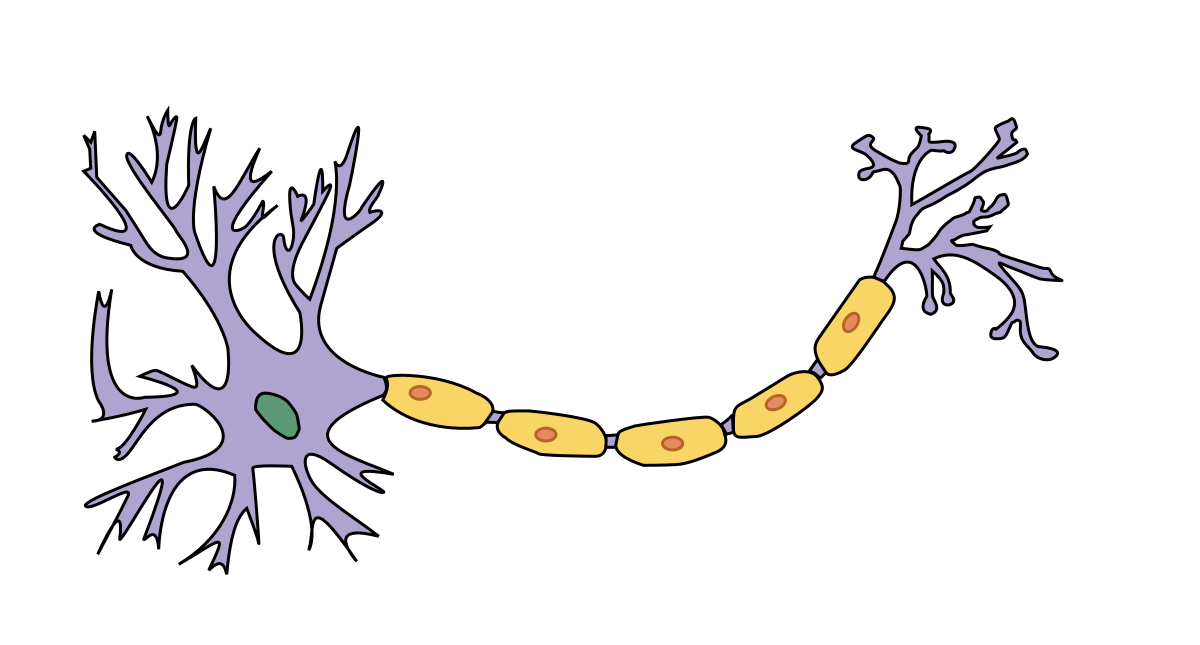
\includegraphics[width=0.8\textwidth]{neuron}
    \caption{Schematic representation of a neuron. \\
    {\small Image from \cite{WikimediaCommonsNeuron}}}
\end{figure}

One of the earliest models for neuronal activity is the \emph{McCulloch-Pitts model} \cite{McCulloch1943}, introduced in 1943. At the time, the understanding of how these cells work was limited, so the two researchers assumed that a neuron can have only one of two possible states (resting or firing). This led them to conclude that the activity of the whole brain could be modelled using propositional logic.

% TODO: finish talking about biological neurons

% TODO: talk about Hebb's rule for learning, Long-Term Potentation and Depression, more modern developments

\subsection{The Perceptron}

In 1957, while working at the Cornell Aeronautical Laboratory, the psychologist Frank Rosenblatt constructed what is widely considered to be the first learning machine to employ an artificial neural network \cite{Rosenblatt1957}.

% TODO: read the original paper (https://www.cs.cmu.edu/~./epxing/Class/10715/reading/McCulloch.and.Pitts.pdf) and cite it (https://link.springer.com/article/10.1007/BF02478259)

% TODO: talk about Rosenblatt's original perceptron algorithm (https://en.wikipedia.org/wiki/Perceptron)
% TODO: cite https://blogs.umass.edu/brain-wars/files/2016/03/rosenblatt-1957.pdf

Inspired by the simple McCulloch-Pitts model, Rosenblatt envisioned a neuron as performing a linear mapping on its inputs and then applying a threshold to determine if it should ``fire''.

\begin{definition}
The \emph{perceptron} is a binary classifier \(P \colon \reals^n \to \Set{0, 1}\) given by
\[
    P_{w, \, b} (x) = \begin{cases}
        1, \text{ if } w \cdot x + b \geq 0 \\
        0, \text{ otherwise}
    \end{cases}
\]
where \(w \in \reals^{1 \times n}\) and \(b \in \reals\) are trainable parameters, learned from the data.
\end{definition}

A neuron under the perceptron model would learn using the following algorithm:
\begin{enumerate}
    \item Choose a \emph{learning rate} \(\alpha > 0\) and initialize \(w\) and \(b\) to some (small) random values, or to zero.
    
    \item For each example \(\left(x, y\right)\) in the training data:
    \begin{itemize}
        \item Compute the current response of the neuron: \(\widehat{y} = P_{w, b} (x)\)

        \item Update the weights accordingly: \(w \xleftarrow{} w + \alpha (y - \widehat{y}) \cdot x\)
    \end{itemize}
\end{enumerate}

% TODO: discussion on a perceptron's mistake bounds: https://arxiv.org/pdf/1305.0208.pdf

Rosenblatt also considered networks with several layers of neurons, but at the time he could not find a working algorithm for training them.

% \subsection{Ivakhnenko's GMDH}

% In parallel with the developments in America, the Soviet-Ukrainian mathematician Alexey Ivakhnenko became interested in the theory of automatic control and developed the \emph{group method of data handling} (GMDH), which could accurately be described as the first instance of training a deep (neural) network.

% TODO: talk about Group Method of Data Handling https://en.wikipedia.org/wiki/Group_method_of_data_handling

% TODO: quote Ivachenko's paper, http://gmdh.net/articles/history/polynomial.pdf

\subsection{Deep Neural Networks}

\begin{definition}
A fully-connected \emph{layer} in a neural network is a  parameterized function
\begin{align*}
    f_{W, \, b} &\colon \reals^d \to \reals \\
    f_{W, \, b} (x) &= h\left(W x + b\right)
\end{align*}
where \(W \in \reals^d, b \in \reals\) are the \emph{layer weights} and \(h \colon \reals \to \reals\) is a non-linear \emph{activation function}.
\end{definition}

\begin{definition}
A feed-forward \emph{artificial neural network} is a parameterized function \(f_{\theta}\) obtained by composing several layers:
\[
    f_{\theta} (x) = f^{(n)}_{W_n, \, b_n} \left(\dots f^{(2)}_{W_2, \, b_2} (f^{(1)}_{W_1 \, b_1} (x))\right)
\]
\end{definition}

% \subsubsection{Backward propagation of errors}

The most commonly used algorithm for training neural networks with (multiple) hidden layers is the \emph{backward propagation of errors}. It was popularized by Rumelhart, Hinton and Williams in a paper from 1986 \cite{Rumelhart1986}, and versions of it have since been used ubiquitously.

% TODO: describe backprop algorithm, chain rule etc.

% TODO: talk about issues during training, instability, saddle points and so on

% \subsubsection{NNs as Universal Function Approximators}

% TODO: talk about the original version of the universal approximation theorem, and then some other variations
% https://en.wikipedia.org/wiki/Universal_approximation_theorem
